\section{Flat combining}
\label{sec:flatco}

This section shows how PCMs in general, and histories in particular,
can formalize the concurrent algorithm design pattern of helping,
whereby one concurrent thread may execute code on behalf of
another. We use Hendler \etal's flat combining algorithm as an
example~\cite{Hendler-al:SPAA10}.  Unlike other proofs of this
algorithm~\cite{Cerone-al:ICALP14,Turon-al:ICFP13}, we don't require
any additional logical infrastructure aside from ordinary auxiliary
state, represented by a
PCM~\cite{LeyWild-Nanevski:POPL13,Nanevski-al:ESOP14}.
%
%This algorithm has been verified
%before~\cite{Cerone-al:ICALP14,Turon-al:ICFP13}, but we illustrate
%that the proof can be developed in a
%
We verify the algorithm \wrt~a generic PCM, and then instantiate with
the PCM of histories. Thus, our proof is usable even in examples where
the specs don't rely on histories. 
%(\eg, the incrementor~\cite{Nanevski-al:ESOP14}).

The flat combiner structure (FC) generalizes a coarse-grained
lock~\cite{Owicki-Gries:CACM76,Nanevski-al:ESOP14,OHearn:TCS07}. In
the case of a lock, threads acquire exclusive access to the shared
resource protected by the lock, \emph{in succession}. With the flat
combiner, threads register the work that they want to perform over the
shared resource. The lock-acquiring thread (aka.~the \emph{combiner})
then executes all the registered work, so the other threads don't need
to compete for the lock anymore. This reduces the contention on the
lock, and improves performance.


\begin{wrapfigure}[13]{r}{4.7cm} 
\centering 
{\scriptsize
%
\begin{minipage}[l]{4.7cm}
\begin{alltt}
\num{ 1} flatCombine(f: \(A{}\to{}B\), x: \(A\)): \(B\) \{
\num{ 2}  \act{reqHelp}(tid, f, x);          
\num{ 3}  \textbf{fix} loop() \{       
\num{ 4}   locked <- \act{tryLock}(); 
\num{ 5}   \textbf{if} locked \textbf{then} \{
\num{ 6}    \textbf{for} i\(\in\!\set{0, \ldots, n-1}\) \{
\num{ 7}     req <- \act{readReq}(i);
\num{ 8}     \textbf{if} req == \textsf{Req} fi xi \textbf{then} \{         
\num{ 9}      w <- fi(xi);    
\num{10}      \act{doHelp}(i, w);
\num{11}     \}\}
\num{12}    \act{unlock}();\}
\num{13}  rc <- \act{tryCollect}(tid);
\num{14}  \textbf{if} rc == \textsf{Some} w 
\num{15}  \textbf{then} \textbf{return} w;
\num{16}  \textbf{else} loop();\}();\}
\end{alltt} 
\end{minipage} 
%
}
\caption{Flat combining algorithm.}
\label{fig:flatco}
\end{wrapfigure}
%
The higher-order \code{flatCombine} procedure
(Figure~\ref{fig:flatco}) works as follows.\footnote{For simplicity,
  we consider a modified version of the original algorithm. In
  particular, (a) we use an array rather than a priority queue for
  registration of help requests, and (b) we don't expunge help
  requests that haven't been served for sufficiently long time.} It
takes as input a \emph{sequential} function $f$ and argument $x$, and
registers the invoking thread for help with executing $f\ x$ over the
shared resource. It does so by storing $\Req{\eesc{f}}{\eesc{x}}$ into
the shared \emph{publication} array, at index \code{tid} (line~2),
where \code{tid} is the id of the invoking thread.
%
It next enters the main loop (line~3) and tries to acquire the lock to
the shared heap (line~4).
%
The acquiring thread becomes a combiner (line~5); it traverses the
publication array, where the global variable $n$ bounds the number of
threads, checking for help requests (lines 6--11). For each request
found (which can arrive even while the combiner holds the lock), the
combiner executes the appropriate function with the provided arguments
(line~9) over the shared heap. It informs the requesting thread
\code{i} of the result \code{w}, by writing $\Resp{\eesc{w}}$ into the
slot \code{i} of the publication array (line~10).
%
After the traversal, the combiner releases the lock (line~12).
%
Finally, the thread (combiner or otherwise), checks the publication
array to see if it has been helped (line~13). If so, it extracts the
result \code{w} from its slot in the publication array, and fills the
slot with $\Done$ (all line~13). The result of the help, if one
exists, is returned in line~15. Otherwise, the thread loops for help
again.

To supply the intuition behind the spec for FC, we first review how
ordinary locks work with auxiliary state, in the subjective setting of
FCSL~\cite{Nanevski-al:ESOP14}. In CSL~\cite{OHearn:TCS07}, and the
Owicki-Gries method~\cite{Owicki-Gries:CACM76}, a lock comes with a
resource invariant $I$ that restricts the heap of the shared
resource. Such restriction implicitly assumes a presence of
``hard-coded'' auxiliary state, describing the contents of the
corresponding shared heap (the explicit parametrization over the
auxiliary state, which we make use of here, is explained in the
introduction of~\cite{LeyWild-Nanevski:POPL13}). When the lock is not
taken, the shared heap satisfies $I$. When the lock is taken, the heap
is in the exclusive possession of the acquiring thread, which can
invalidate $I$, but has to restore it before releasing the lock. The
subjective setting is similar, except the values of the auxiliary
state are drawn from a PCM $\pcmS$, and specs keep track of two values
$\gS$ and $\gO$, describing how much the thread (\emph{self}) and its
environment (\emph{other}) have contributed to the resource,
respectively. When the lock is free, the heap of the shared resource
satisfies $I(\gS \join \gO)$. When the lock is released by a thread,
the thread may update its $\gS$ by some value $\gd$, reflecting that
its contribution to the resource changed. Thus, if before locking, the
resource satisfied $I(\gS \join \gO)$, after unlocking it will satisfy
$I(\gS \join \gd \join \gO)$, as shown by examples in Section~3
of~\cite{Nanevski-al:ESOP14}.

The setup of the flat combiner is similar, but in addition to $\gS$
and $\gO$, FC also keeps an array $\gp$ storing a $\pcmS$-value for
each thread. The entry $\gp[i]$ signifies how much the thread $i$ has
been helped by the combiner. If $\gp[i]=\gd$ is non-unit, $i$ can
collect the help by joining $\gd$ to its own $\gS$, and setting
$\gp[i]$ to the unit $\pcmU$ of $\pcmS$, after which it can ask for
help again. Thus, the overall relation between the auxiliary state and
the resource heap, when the lock is free, is captured by the invariant
$I~(\jjoin{i}\gp[i] \join \gS \join \gO)$.

\subsection{Flat combiner state and transitions}

The states of the FC concurroid $\fccon$ are described by the assertion:
% 
%\vspace{-5pt}
%
\[
%\tag{\arabic{tags}}\refstepcounter{tags}\label{eq:fc-state}
{\small
\begin{array}{c}
  W_{\fccon} \!\eqdef\! 
  \hfc \spts (\tS, \mS, \gS) \aand 
  \hfc \opts (\tO, \mO, \gO) \begin{array}[t]{l}
    \hbox{}\aand \hfc \jpts {\angled{\lk \hpts b \hunion h_p \hunion h_r, \gp}} \aand \exists l_p\ldot \Array{\ap}{n}{l_p}{h_p} 
\end{array}
\end{array}
}
\]
%
The auxiliary state in the self/other components consists of the
following. $\tS$ and $\tO$ are sets of thread ids, which form a PCM
under disjoint union.\footnote{One thread may hold many thread id's,
  which it distributes between its children upon forking.}
%
$\mS$ and $\mO$ are elements of the \emph{mutual exclusion} set $O =
\{\lockNown,
\lockOwn\}$~\cite{LeyWild-Nanevski:POPL13,Nanevski-al:ESOP14} and
record whether the lock $\lk$ is owned by the thread, or the
environment. $O$ is a PCM under the operation defined as $x
\join \lockNown = \lockNown \join x = x$, with $\lockOwn \join
\lockOwn$ undefined. The unit element is $\lockNown$, and the
undefinedness of $\lockOwn \join \lockOwn$ means that two threads
can't simultaneously own the lock.
%
$\gS$ and $\gO$ are elements of a generic PCM $\pcmS$, as
described above.
% 
The self/other triples form a PCM with component-wise lifted joins
and~units.
 
The joint component of $\fccon$ contains a concrete heap, and the
auxiliary array $\gp$.
%
The concrete heap keeps the pointer $\lk \hpts b$, which stands for
the lock, with the boolean $b$ representing the lock status. It also
stores the publication array with the origin pointer $\ap$ into the
heaplet $h_p$ (see notation~\eqref{eq:array}). The array stores
elements of type $\mathsf{Stat} \eqdef \Done~|~\Req{f}{x}~|~\Resp{w}$,
as already apparent from Figure~\ref{fig:flatco}.  We abuse the
notation and refer to the array represented by $h_p$ as $\ap$.
%
The heap $h_r$ is the resource protected by the FC lock. Upon locking
it moves to the exclusive ownership of the combiner. 

%The array $\gp$ stores the auxiliary state obtained by helping. When
%the combiner executes \code{fi} on behalf of $i$, the execution should
%influence not only the locked heap, but also the auxiliary $\gS$ of
%the thread $i$. However, the combiner can't change the self components
%of other threads. Thus, it records into the $i$-th entry of the joint
%auxiliary array $\gp$ a value $\gd$ obtained as an auxiliary value
%after the call to $\code{fi}$. The thread $i$ eventually collects this
%value, and joins it with its own $\gS$.

%The FC concurroid comes with a resource invariant $I$, similar to
%CSL~\cite{OHearn:TCS07}. $I$ is predicate relating the resource heap
%$h_r$, with the auxiliaries $\gS$ of the various threads, thus
%allowing threads to reason about the resource heap abstractly in terms
%of $\gS$'s. 
We further assume the following properties of $W_{\fccon}$:
%
\begin{itemize}
\item [$(i)$] for any $\tid$, if $\gp[\tid] \neq \pcmU$, then $\ap[\tid] =
  \Resp{w}$ for some $w$;
\item [$(ii)$] if $b$ is $\True$ then $\h_r = \hempty$ and $\mS \join
  \mO = \lockOwn$; otherwise $\mS \join \mO = \lockNown$ and
  $I~(\jjoin{i}\gp[i] \join \gS \join \gO )~h_r$.
\end{itemize}
%
Property $(i)$ ensures that the auxiliary array $\gp$ holds a pending
contribution in a cell $\tid$ only if the corresponding entry in the
publication array $\ap$ points to the response with some (uncollected)
result.
%
Property $(ii)$ formally relates the auxiliary state to the resource
heap $h_r$, as already described.

Flat combiner concurroid's external transitions intuitively correspond
to locking and unlocking the heap $h_r$, thus moving it from the joint
to private state, and vice-versa. We don't present them formally, as
they are similar to the transitions in CSL~\cite{Nanevski-al:ESOP14}.
%
The internal transitions $\reqtrans$, $\helptrans$ and $\colltrans$
synchronously change the contents of $\ap$ and $\gp$ for a particular
thread id $i$ (one at a time) as the following diagram illustrates.
%
%\vspace{5pt}
%
\begin{center}
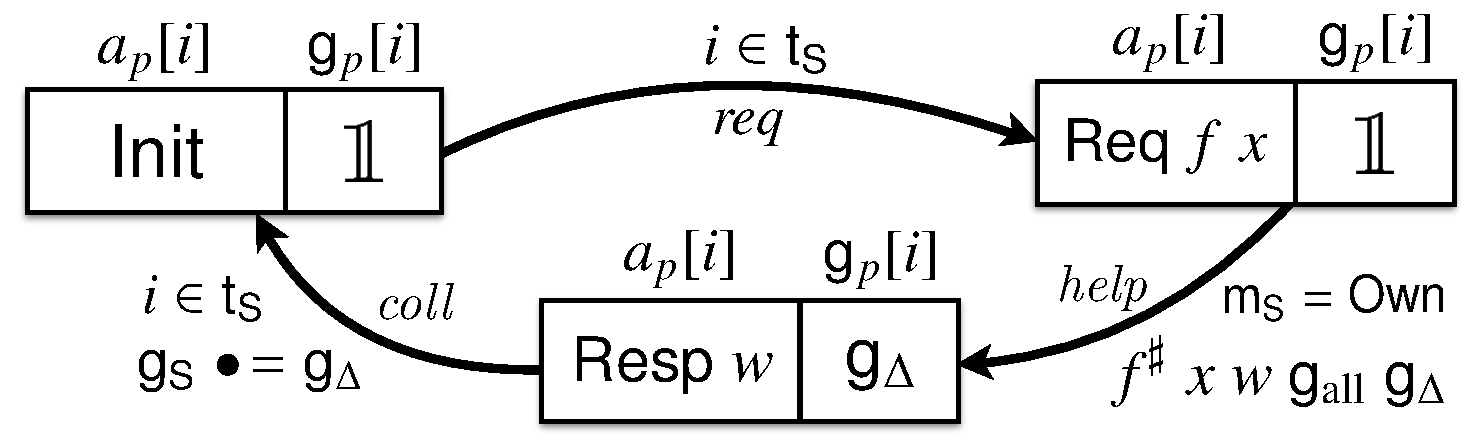
\includegraphics[width=0.60\textwidth]{fctrans.pdf}    
\end{center}
%
%\vspace{5pt}
%
The transition $\reqtrans$ can be taken only by a thread holding the
thread id $i$; it changes the value of $\ap[i]$ from $\Done$ to
$\Req{f}{x}$ for some $f$ and $x$.
%
The transition $\helptrans$ can be performed by any thread that owns
the lock (not necessarily the one with the id $i$); it replaces the
contents of $\ap[i]$ and $\gp[i]$ with an appropriate result $w$ and
an auxiliary delta $\gd$, respectively. The two are valid \wrt~the
input $x$ and the cumulative auxiliary $\gall$, as ensured by the
constraint $\fspec{f}$.
%
Finally, $\colltrans$ is invoked by the thread with id $i$; it flushes
the contents of $\gp[i]$, into the self-contribution $\gs$ and puts
$\Done$ into $\ap[i]$.

\subsection{Flat combiner specification}
\label{sec:fc-conc-spec}


We now provide a spec for \code{flatCombine} in terms of the
concurroid $\fccon$. We assume $f : A \to B$, $x : A$, and $f$ comes
with the following spec.\footnote{Thus, we don't require $f$ to be
  sequential (\ie, in addition to just manipulating the
  privately-owned state, $f$ can also allocate new concurroids via
  hiding, and fork children threads), but every sequential function
  can be given a spec in~$\privcon$.}
%
\[
\tag{\normalsize \arabic{tags}}\refstepcounter{tags}\label{eq:fspec}
{\small
\hspace{-5pt}
\begin{array}{c}
\sspec{~
\exists h\ldot \hpriv \spts h \aand I~\g~h
~} 
~~f(x)~~
\sspec{~
\exists h'~\gd\ldot\hpriv \spts h' \aand I~(\g \join \gd)~h' \aand
\fspec{f}~x~\res~\g~\gd
~}@\privcon
\end{array}
}\]
%
The spec allows the input heap $h$ to change to $h'$. The resource
invariant $I$ has to be preserved, up to a change of the auxiliary
state, from $\g$ to $\g \join \gd$. $\fspec{f}$ is a client-supplied
predicate which specifies $f$. We call it \emph{validity predicate};
it's functional with respect to~$\gd$, and relates the input value
$v$, the result value~$\res$, the initial auxiliary state~$\g$ and the
``auxiliary delta'' $\gd$ resulting from the invocation of~$f$.
%
For instance, if $f$ were a sequential push operation on stacks, with
$\g$ and $\gd$ being set to histories $\hist$ and $\histd$, we might
choose the following validity predicate:
%
\[
\tag{\normalsize \arabic{tags}}\refstepcounter{tags}\label{eq:push-spec}
{\small
%\hspace{-4.1mm}
\begin{array}{r@{\ }c@{\ }l}
  \fspec{\push}~x~\res~\hist~\histd & \eqdef & \res = () \aand \histd =
  \tfr{\hist} \hpts (l, x::l),
\end{array}
}\] 
%
where $l = \hist[\last{\hist}]$. That is, $\fspec{\push}$ fixes the
result of $\push$ to be unit and its effect to be the singleton
history describing the action of pushing.

%
%We require that $f$ preserves the invariant $I$. 
%The  operates over the private heaps only, it can be
%considered as sequential. 
%spec~\eqref{eq:fspec} is indeed sequential, as it captures only
%elements of the privately-owned heap and can possibly make use of the
%unconstrained allocator.

For the \code{flatCombine} spec, we need two auxiliary predicates.
$\NoReqs$ indicates that the thread $\tid$ doesn't request
help. $\histso{\cdot}{\cdot}$, generalizes~\eqref{eq:histso} from
histories to PCM~$\pcmS$.
%
\[
\tag{\normalsize \arabic{tags}}\refstepcounter{tags}\label{eq:noreqs}
{\small
\begin{array}{rcl}
\noreqs{\tid} & \eqdef & \hfc \spts (\set{\tid}, \lockNown, -) \aand
\ap[\tid] = \Done     
\\[5pt]
\histso{\hfc}{\gS, \gO, \g} & \eqdef &\hfc \spts  (-, -, \gS)
  \aand 
\hfc \opts (-, -, \gO) \aand
\g \pre \jjoin{i}\gp[i] \join \gS \join \gO    
\end{array} 
}
\] 
%
%\hspace{-5pt}
%
Here, the partial order $\pre$ on PCM elements is defined as $\g_1
\pre \g_2 \eqdef \exists \g, \g_2 = \g_1 \join \g$. It generalizes the
relation $\pre$ from histories to the PCM $\pcmS$, and in the
specs captures that the value $\g_1$ was ``current'' before $\g_2$.
%

The spec for \code{flatCombine} is given \wrt a specific thread id
$\tid$.
%
%\vspace{-5pt}
%
\[
\tag{\normalsize \arabic{tags}}\refstepcounter{tags}\label{eq:fc-spec}
{\small
\hspace{-10pt}
\begin{array}{c}
\spec{
  \hpriv \spts \hempty ~\sep~ \histso{\hfc}{\pcmU, -, \g} \aand
  \noreqs{\tid} 
} 
\\
\eesc{flatCombine}(f, x): B
\\
\spec{
\begin{array}{c}
\exists \g'~\gd\ldot \hpriv \spts \hempty ~\sep~
\histso{\hfc}{\gd, -, \g'} \aand \noreqs{\tid} \aand 
\g \pre \g' \aand
\fspec{f}~x~\res~\g'~\gd 
\end{array}
}@\privcon\entangle\fccon
\end{array}
}
\]
%
%
A call to \code{flatCombine} starts and ends in a state in which the
thread $\tid$ doesn't request the help ($\NoReqs$), and in which $\g$
names the sum total of the contributions. It doesn't change the
privately-owned heap, but increases self-contribution by amount of an
auxiliary delta $\gd$. The mediating value $\g'$ is a sum-total of the
contributions at the moment when the thread received help; thus,
$\fspec{f}~x~\res~\g'~\gd$. As $\g'$ is current sometime after the
initial $\g$, the spec postulates $\g \pre \g'$.
%
%relating the input and result values with $\gd$ using $\fspec{f}$:
%$\g'$ captures the overall auxiliaries combined at \emph{some moment}
%during the execution of \code{flatCombine}. Using $\g$ for this
%purpose would make the postcondition non-stable.
%
Due to space limitations, we omit a detailed discussion on
verification of the spec~\eqref{eq:fc-spec} of the flat combiner (it
can be found in Appendix~\ref{sec:verifying-fc} or in the accompanying
Coq files).

To strengthen the analogy with coarse-grained CSL-style locks, let us
note that if one were to implement a procedure
$\eesc{coarseGrainedCombine}(f, x)=\eesc{\{}
\eesc{lock}();~f(x);~\eesc{unlock}() \eesc{\}}$, its specification
would be the same as~\eqref{eq:fc-spec}, modulo the $\NoReqs$ conjunct
and the join with all $\gp[i]$ components in \eqref{eq:noreqs}, which
would not be present in the coarse-grained case, as they are artefacts
of the helping machinery.\footnote{To provide truly \emph{the same}
  specs, one would need to introduce abstract predicates to hide these
  artefacts, but we can do that in Coq, so we omitted the discussion
  on them in this paper.}

\subsection{Instantiating the flat combiner for stacks}
\label{sec:instantiating-fc}

To illustrate that the abstract spec for the flat combiner follows the
expected intuition, we consider an instance where $\gS, \gO, \gp$ are
histories, and $f$ is the sequential \code{push} method for stacks,
satisfying~the generic sequential spec~\eqref{eq:fspec} with the
validity predicate $\fspec{\push}$ defined by~\eqref{eq:push-spec} and
the stack invariant~\eqref{eq:tb-states}.
%
%A sequential implementation of $\push$ would come with the following
%accompanying validity predicate $\fspec{\push}$:
%
%
%\[
%\tag{\normalsize \arabic{tags}}\refstepcounter{tags}\label{eq:push-spec}
%{\scriptsize
%%\hspace{-4.1mm}
%\begin{array}{r@{\ }c@{\ }l}
%  \fspec{\push}~x~w~\hist~\histd & \eqdef & w = () \aand \histd =
%  \tfr{\hist} \hpts (l, x::l),
%\end{array}
%}\]
%%
%where $l = \hist[\last{\hist}]$. That is, $\fspec{\push}$ fixes the
%result of $\push$ to be unit and its effect to be the singleton
%history describing the ``push''. 
%
So by instantiating~\eqref{eq:fc-spec}, after some simplification, we
obtain:
%
\[
\tag{\normalsize \arabic{tags}}\refstepcounter{tags}\label{eq:fc-push-spec}
{\small
\begin{array}{c} 
\spec{
\begin{array}{c} 
  \hpriv \spts \hempty ~\sep~
  \histso{\hfc}{\hempty, -, \hist} \aand
  \noreqs{\tid} 
\end{array}
} 
\\
\eesc{flatCombine}(\push, e): \mathsf{Unit}
\\
\spec{
\begin{array}{c}
\exists t~l\ldot \hpriv \spts \hempty ~\sep~
\histso{\hfc}{t \hpts (l, e::l), -, \hist} \aand
\hist < t \aand
\noreqs{\tid}
\end{array}
}
%@(\privcon\acon)\entangle\fccon
\end{array}
}
\]
%
Note that~\eqref{eq:fc-push-spec} is very similar to the spec
\eqref{eq:stack-spec} for Treiber \code{push}; the only difference,
again, is in the FC-specific components such as thread id's, the
$\NoReqs$ predicate, and the lock status views used in the definition
of $\NoReqs$. Thus, the spec~\eqref{eq:fc-spec} is adequate.
%
A similar derivation can be done for an FC-specification of $\pop$.

